\documentclass[border=10pt]{standalone}
\usepackage{pgfplots}
\pgfplotsset{compat=1.18}
\begin{document}
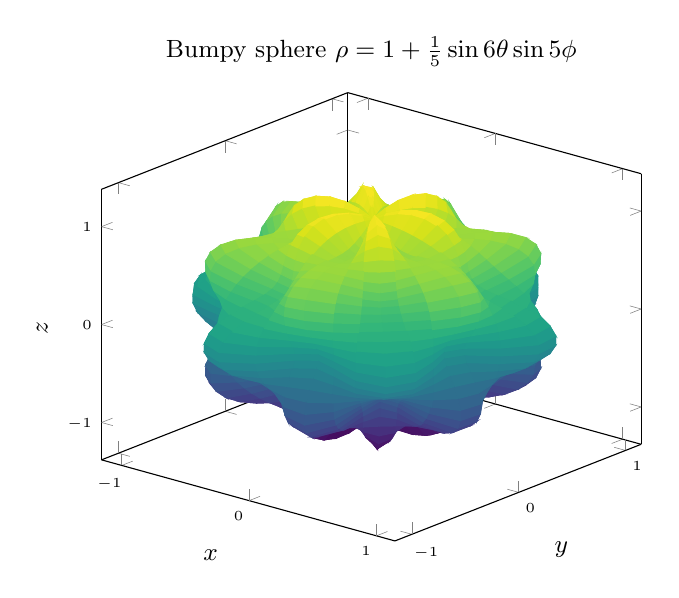
\begin{tikzpicture}
\begin{axis}[
    view={40}{25},
    domain=0:360, samples=40,
    y domain=0:180, samples y=40,
    z buffer=sort,
    colormap/viridis,
    xlabel={$x$}, ylabel={$y$}, zlabel={$z$},
    title={Bumpy sphere $\rho=1+\frac15\sin 6\theta\sin 5\phi$},
    tick label style={font=\tiny},
    label style={font=\small},
    title style={font=\small},
]
\addplot3[surf, shader=flat, point meta=z]
(
  {(1+0.2*sin(6*x)*sin(5*y))*sin(y)*cos(x)},
  {(1+0.2*sin(6*x)*sin(5*y))*sin(y)*sin(x)},
  {(1+0.2*sin(6*x)*sin(5*y))*cos(y)}
);
\end{axis}
\end{tikzpicture}
\end{document}